% !TeX root = ../main.tex
% Add the above to each chapter to make compiling the PDF easier in some editors.

\chapter{Experiments}

In total, 5 experiments were conducted for this thesis. Two were quick proof-of-concept experiments to validate the initial speculation, two - pilot studies to determine values for some properties of the final experiment and test the process of sampling participants on \gls{wa} index, and one formal study to test \nameref{final_study}.


\begin{comment}
\section{Prototypes/Proof of concept}

Initial motivation for this work was a question of whether sudden manipulations of buildings in \gls{vr} would cause uncomfortable experience for users (Fig. \ref{fig:a1unawareofa2actions}). Two prototypes were developed to test this speculation, these are described in the Buildings Popping Up and Moving Buildings paragraphs.

\begin{figure}
	\centering
	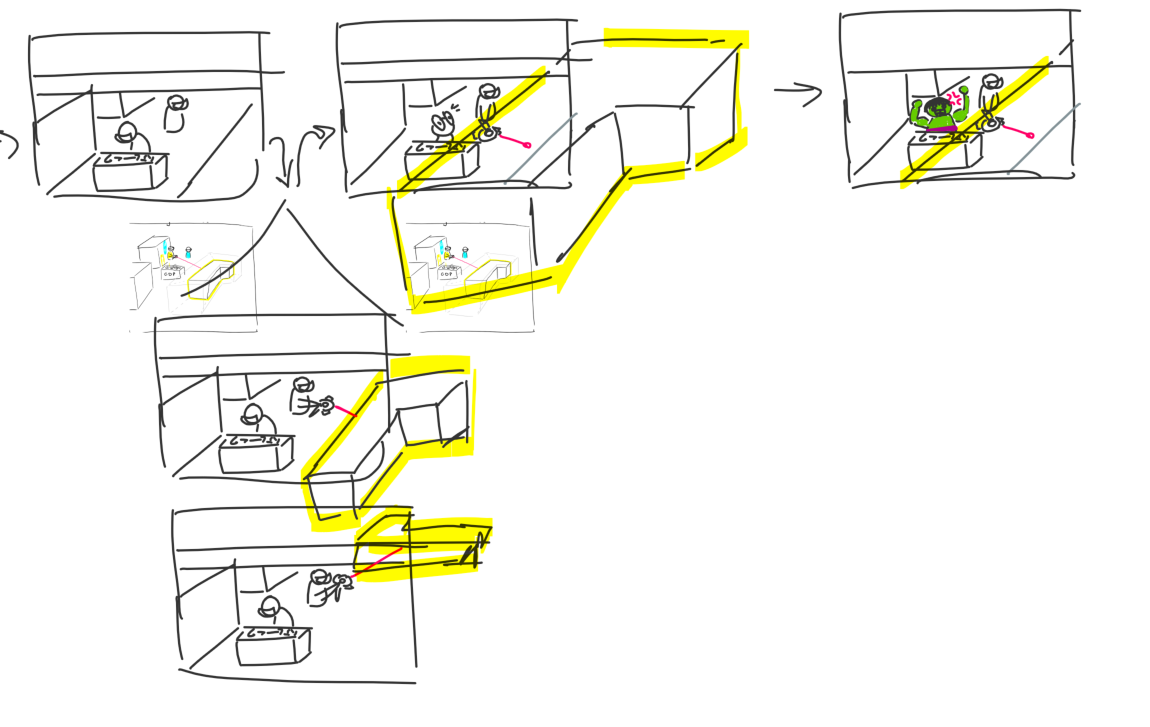
\includegraphics[width=0.7\linewidth]{figures/placeholders/A1_unaware_of_A2_actions}
	\caption{Collaborators unaware of each other's actions}
	\label{fig:a1unawareofa2actions}
\end{figure}

\paragraph{Buildings Popping Up} 
\label{buildingspoppingup}
The first prototype looked into how the participants' experience would be influenced, if a building suddenly appeared in-front of them, when they were occupied with their own task.

% Participants
3 participants (all male) were chosen among the members of the \gls{hci} group at the University of Otago. Two had prior experience in \gls{vr}, one had not.

% Procedure & Task
Participants were placed in the immersive \gls{vr} environment: a 3D model of the campus of the University of Otago. This was not a collaborative task, the participants were in the \gls{ve} alone. First, the the affordances of the environment were introduced (teleportation, walking and looking around), then participants were asked to navigate to the university clock tower. During this navigation task, a building would pop up in-front of them a couple of times at pseudo-random times (decided and initiated by the experimenter). After the completion of the experiment the participants were asked to describe the experience, especially the parts, where a building appeared in-front of them.

% Apparatus (i.e Unity, Resonance Audio, stereo headphones, Vive)
Unity3d and Oculus Rift \gls{hmd} with Touch Motion controllers were used in this experiment.

% Results
The participant with no prior experience in \gls{vr} described the experience as unexpected, but was also not sure, whether he caused it. The other two participants indicated that they were a bit stuttered by the experience, but in general, "didn't care much for it". Additionally, the participants described the experience as irritating, when the building continued to repeatedly appear after the first encounter.
% Limitations
% I do not check if anyone is concerned with the moving buildings when they get used to it.
% This doesn't matter tho, because according to the WA, people should know what the others are doing in the same environment.
% Discussion of the results?
%...


\paragraph{Moving Buildings}
Due to the results of the first experiment, the problem was regarded as worthwhile of further exploration. For the second proof of concept, a decision was made to come a bit closer to the initial motivation: buildings moving in \gls{ve}.
% Participants
4 new participant (all male) were chosen among the members of \gls{hci} group at the University of Otago, none took part in the previous experiment. Three had moderate experience with \gls{vr}, one had little.
% Procedure & Task
The environment affordances and the introduction remained the same. The task was extended, so that when participants find the clock tower, they were asked to assume their place at the viewing spot prepared for them (Fig. \ref{fig:prototype2viewvingspot}). At this point the participants were asked to observe the clock tower and tell the experimenter if anything seemed odd about it. Some elements of the tower were off axis (Fig. \ref{fig:prototype2clocktoweroddfeatures}), and this task was meant to lull participants' vigilance. As soon as participants started looking for any odd features, the movement of the clock tower towards the used with the speed of 200 units (meters) per second was initiated by the experimented. The approximate distance to from the viewing spot to the tower was 69 meters, the clock tower would stop 0.5 meters in-front of a participant. At this point the experiment would finish, and the participants would be asked about their experience.
\begin{figure}
	\centering
	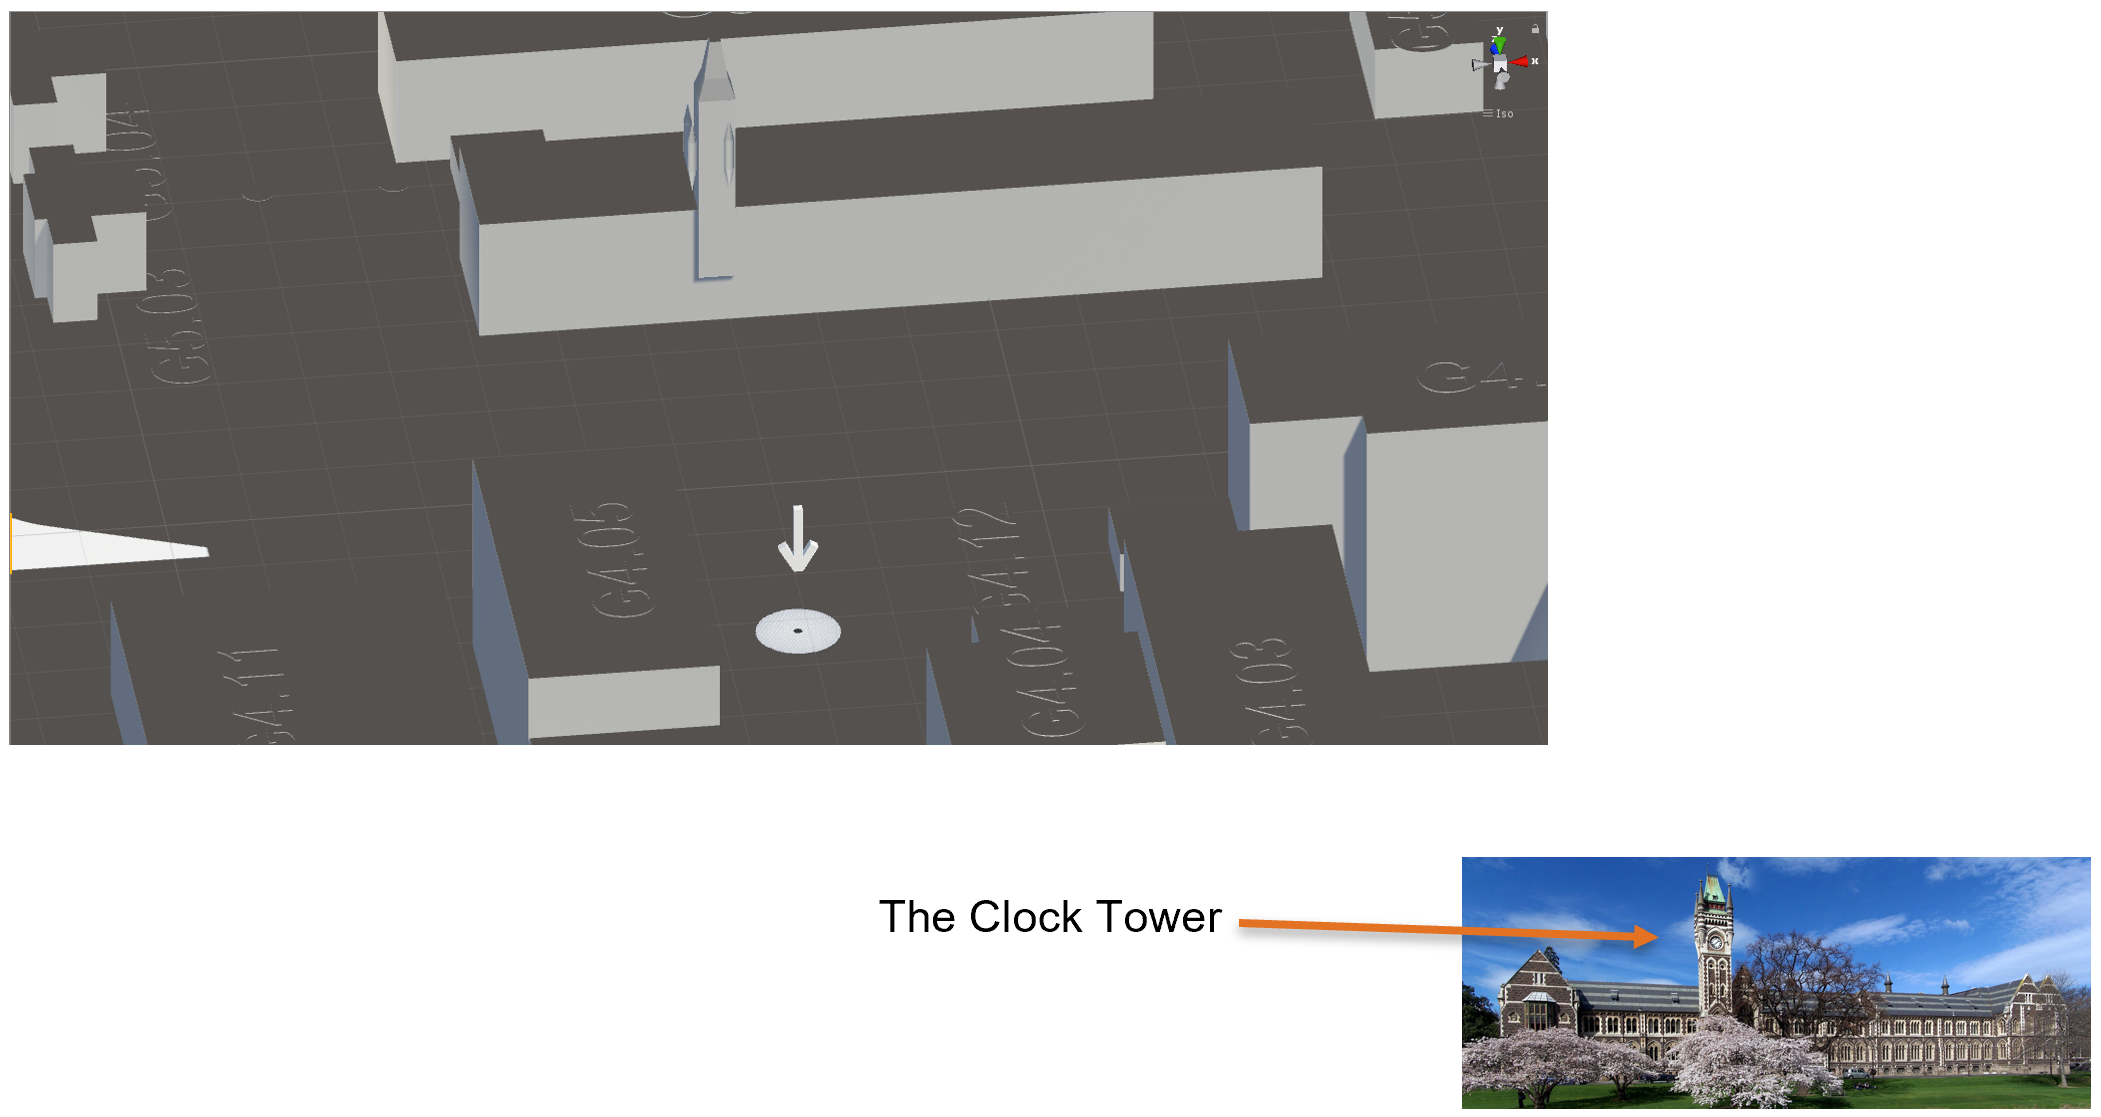
\includegraphics[width=0.7\linewidth]{figures/placeholders/prototype2_viewving_spot}
	\caption{The viewing spot in-front of the university clock tower}
	\label{fig:prototype2viewvingspot}
\end{figure}
\begin{figure}
	\centering
	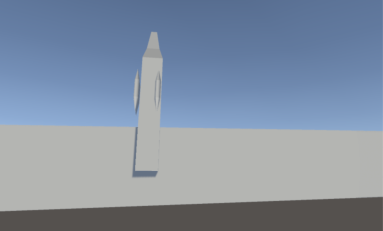
\includegraphics[width=0.7\linewidth]{figures/placeholders/prototype2_clocktower_odd_features}
	\caption{The odd features of the university clock tower model}
	\label{fig:prototype2clocktoweroddfeatures}
\end{figure}
% Apparatus
The same apparatus was used, as in the \nameref{buildingspoppingup} prototype.
% Results

% Limitations
\end{comment}


\section{Pilot Studies}
In preparation to the \nameref{final_study} study, two pilot studies were conducted: \nameref{study_one}, and \nameref{study_two}. This was done to study certain aspects of the final study separately, and make decisions, such as what sound type (earcons or auditory icons) to choose, and at what speed to translate the buildings.

\subsection{Sound Speed and Type}
\label{study_one}
% Goal of the study
Some of the feedback from the initial prototypes indicates that the speed of the moving building was either too fast, or too slow. The goal of this study was to derive the speed participants felt would be appropriate to allow them to perform spatial judgments. Additionally, this pilot study was meant to help determine what type of auditory cues to use: earcons or auditory icons.

\paragraph{Methods}
% Participants
Seven participants (7 men, 1 woman) were chosen among the members of the \gls{hci} group at the University of Otago. One had reported bad hearing, and one had a flu and a "stuffed nose".  None of the participants had any architectural background. Some of the participants were online gamers.
% TODO: figure out the age distribution

% Procedure & Task
The study was carried out in a \gls{ve} that was specifically setup for this purpose (see Fig. \ref{fig:clipimage001}). A participant was placed at the Center of the environment, in which there was a real-sized building that could be translated by the experimenter from and to any of the predefined positions: Left Front (LF), Right Front (RF), Left Back (LB), Right Back (RB), Front (F), Back (B), Left (L), Right (R), Center (C). When the building moved, a sound was emitted from its position. 

The purpose the whole research and this study was explained or reminded to the participants. They were placed at the center of the scene (C) with the building placed in front of them , and asked to preserve the orientation of the chair they were seated upon, but were also told that they were allowed to move their head. 

Participants were put through a tutorial to build a correlation between the visually perceived movements of the building and the emitted sound: the building was translated along the major directions (C-F, C-L, L-R, L-C, C-B), and then additionally between randomly selected positions from the predefined set (Fig. \ref{fig:pilot1predefinedtutorialtranslations}).
For the actual experiment, participants were asked to close their eyes and guess the path that the building traversed. It was silently positioned at a randomly selected position and then translated with auditory cues to a new randomly selected position (see Fig. \ref{fig:pilot1controlpanel}). This was repeated for each type of sound (N=2), and each speed (M=3). 

After going through all the sound types and speeds, participants were asked for their honest opinion, as to which sound was the best, and what speed was the most appropriate. 

\begin{figure}
	\centering
	\includegraphics[width=0.7\linewidth]{C:/Users/bowli/AppData/Local/Temp/msohtmlclip1/01/clip_image001}
	\caption{Experiment setup}
	\label{fig:clipimage001}
\end{figure}

\begin{figure}
	\centering
	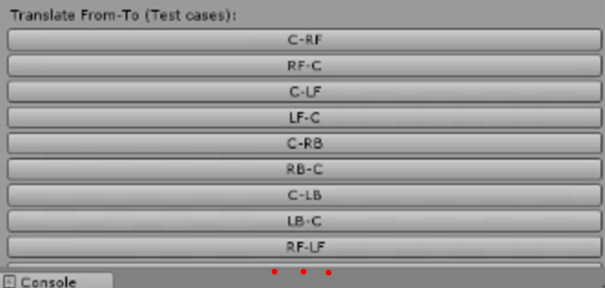
\includegraphics[width=0.7\linewidth]{figures/placeholders/pilot1_predefined_tutorial_translations}
	\caption{Predefined translation paths}
	\label{fig:pilot1predefinedtutorialtranslations}
\end{figure}

\begin{figure}
	\centering
	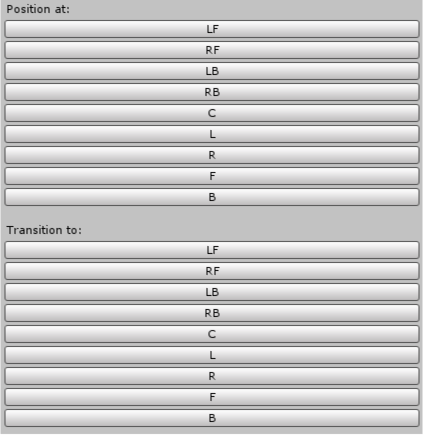
\includegraphics[width=0.7\linewidth]{figures/pilot1_control_panel}
	\caption{Control panel for translations}
	\label{fig:pilot1controlpanel}
\end{figure}


% Apparatus (i.e Unity, Resonance Audio, stereo headphones, Vive)


% Study Factors and Conditions: what my factors are, conditions == independent variables' values
Repeated measurements design

Which sound type was played first was also changed between participants, so that for 4 people the first one was the concrete auditory icon, and for the other - the sine wave "humming" earcon.

Two sounds used in this study were: a sound mimicking a concrete block sliding on another concrete block (auditory icon), and a simple sine wave (earcon).

Positions' selection was pseudo-random and made with some degree of bias to prioritize longer translation paths, so that users have more time to analyze the sound and guess (i.e. the path from RB to LB would be longer, than just RB to B).

% Results

% Discussion

% Limitations


\subsection{Spatial Judgment}
\label{study_two}
\section{Workspace Awareness in Immersive Virtual Reality}
\label{final_study}
% Goal of the study
The goal of this study was to analyze \gls{wa} that participants have of others present in the same immersive \gls{vr} environment. Participants were presented with a primary and secondary tasks. Primary task was tracing 3D models with a 3D brush, and secondary task was a \gls{wa} task - reporting changes to the environment.

\paragraph{Methods}
Aspects of \gls{wa} that were evaluated was participants’ reaction speed when provided with different types of awareness presentation (audio and/or visual cues from the environment).

% Participants
12 participants (8 men and 4 women) were recruited among friends, employees from the chair, and students from the \gls{tum}; ages ranged from 22 to 32 (mean 25.2, std. 2.5). Only one participant reported having "partially" good hearing, others reported good hearing. 3 people reported to be familiar with \gls{vr} technology, among them, one person reported being a proficient gamer and one - having partaken in driving simulator studies. Participants were a mix of gamers, non-gamers, and casual gamers. Participants were also equally distributed among people who had experience with \gls{vr}, those who had some experience, and those who had no prior experience. Two reported being online gamers, and another two - occasional online gamers. Only one person had prior experience with architecture, and had worked in the field. One participant tried 3D drawing in the system, but otherwise none of the participants had seen the system before, or took part in the trial studies.

% Procedure
Participants were given a written and verbal introduction to the experiment,
after which were asked to sign the consent form for using their data.
Next, participants went through the tutorial, where the 3D brush, laser pointer for pinpointing the buildings and auditory cues were introduced. Participants went through a small scenario resembling the actual experiment, where they were asked to trace a pillar, while catching a moving building, and keeping track of how the building sounds and where it is visually.
During the actual experiment, each participant was tested in each of the 3 test groups.
At the end of the experiment, participants were asked to fill in a self-report questionnaire.
Participants did not rest between the different conditions. 

% Task
Participants were tasked with the scenario, in which there are 2 architects (A1 and A2), who perform their separate tasks in the same urban district (\ref{fig:urbandistrict}) in \gls{vr}. A1 (participant) has 2 tasks: primary and secondary. The primary task is to trace given 3D shapes with a 3D brush (a tracked 6-\gls{dof} controller). Meanwhile, A2 (simulated ivisible user) can translate any building in the district to any other part of the district at any time. The secondary (workspace awareness) task of A1 is to keep track of changes to the environment and pinpoint them with a virtual laser pointer (another tracked 6-\gls{dof} controller).

\begin{figure}
	\centering
	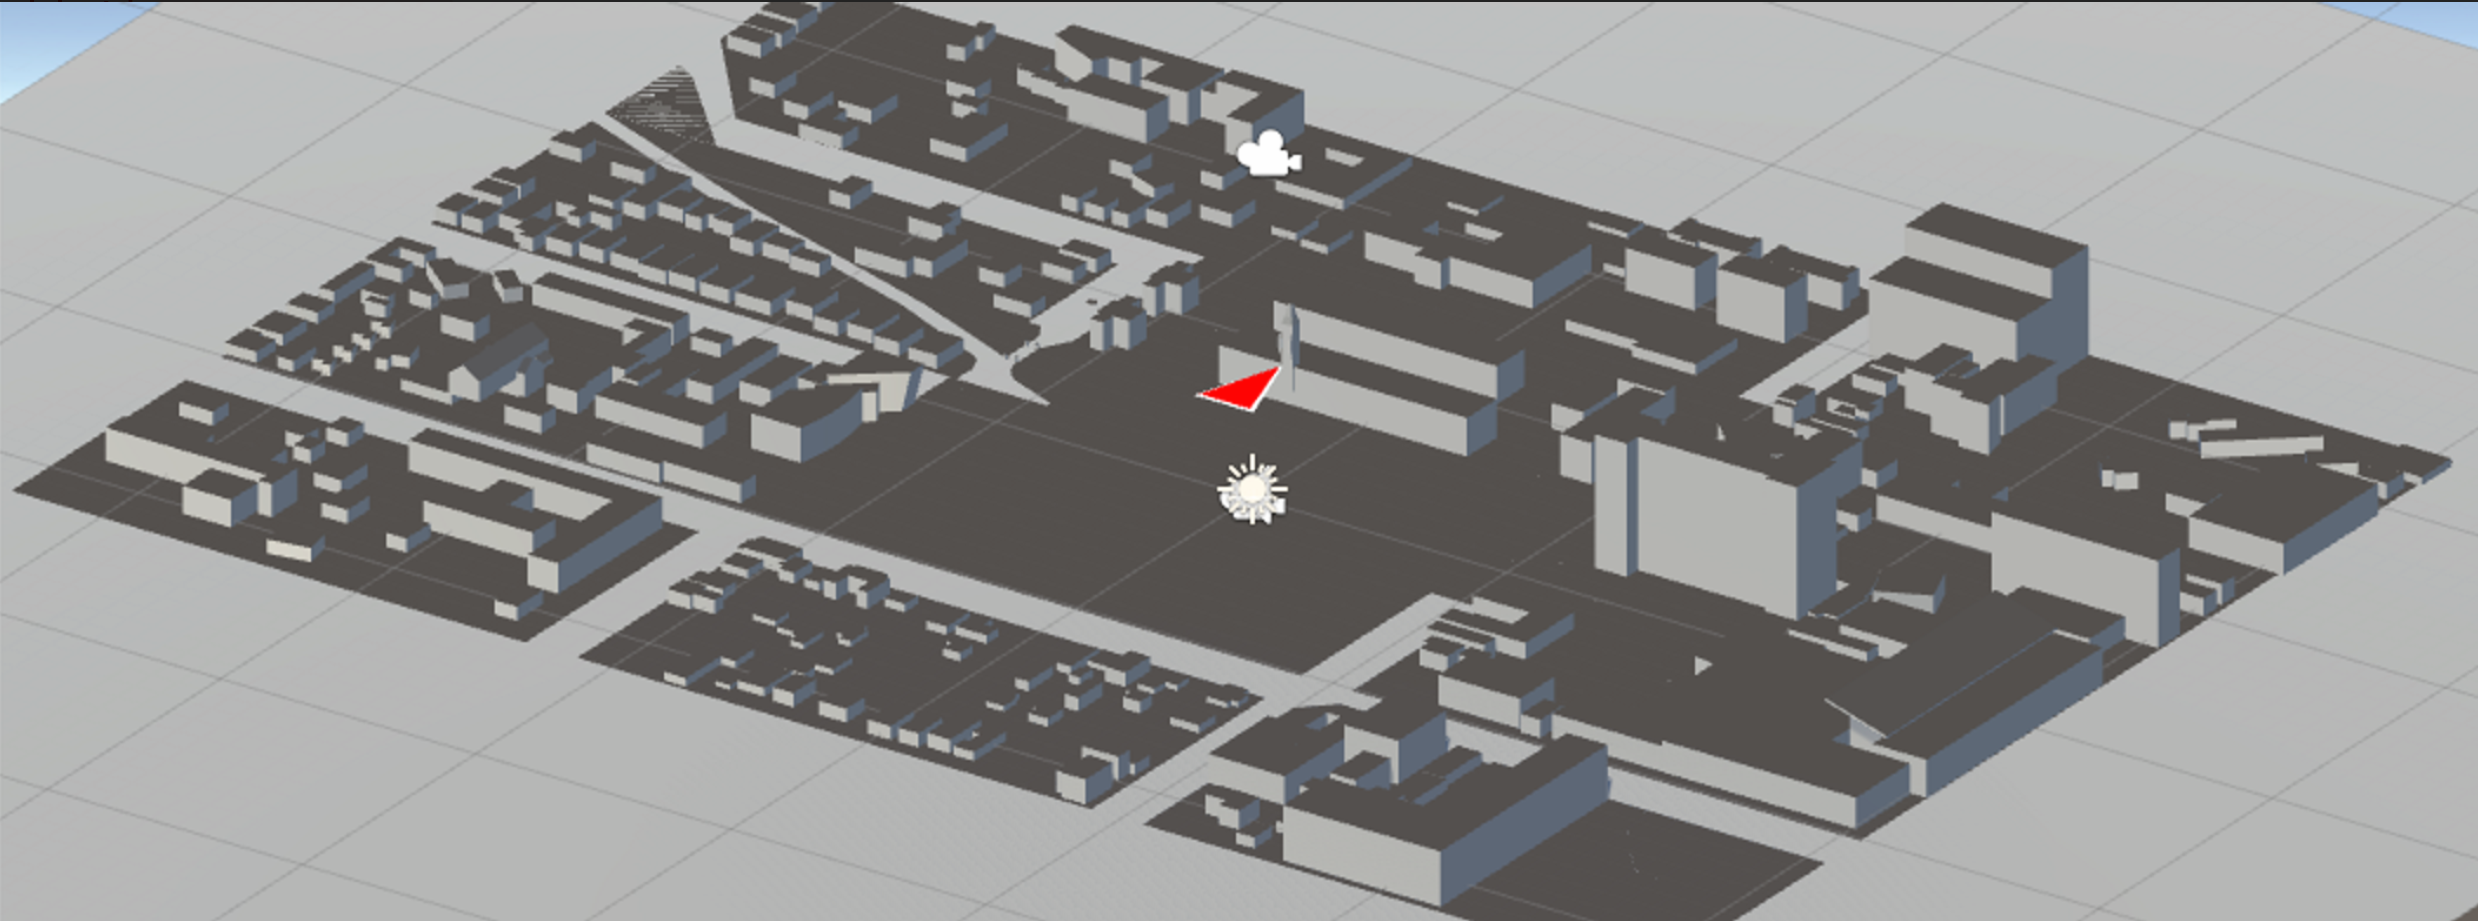
\includegraphics[width=0.7\linewidth]{figures/urban_district}
	\caption{Simulated urban district for the \gls{wa} study}
	\label{fig:urbandistrict}
\end{figure}


% Apparatus: Unity, Resonance Audio, stereo headphones, Vive
Experiment was implemented with the help of Unity3d, version  2018.1.5f1 and Resonance Audio SDK for Unity, version 1.2.1 with sound occlusion turned off. For the hardware, \gls{vr} headset and controllers from the HTC Vive were used, along with on-ear stereo headphones, and a Windows 10 PC (TODO: specs).

% Study Factors and Conditions: what my factors are, conditions == independent variables' values
% + Repeated-measures design?
\textit{Experimental Design} 
The study examined one independent variable: type of awareness presentation. 3 controlled awareness presentations  were made available to the participants: a minimap of the district (\ref{fig:minimap_controller}), auditory cues emitted by translating buildings in the scene (sound of concrete sliding on concrete), and their combination. Awareness presentations were rotated for each participant, so that each presentation was seen in the same position equal number of times. 
Each awareness presentation was tested for 10 minutes, during which exactly 8 buildings were chosen and translated randomly. There were 24 data points measured per user in each session. Data collected were the reaction speed in determining the position of a moving \gls{vb}, along with 3D drawings created by participants.

\begin{figure}[h]
	\centering
	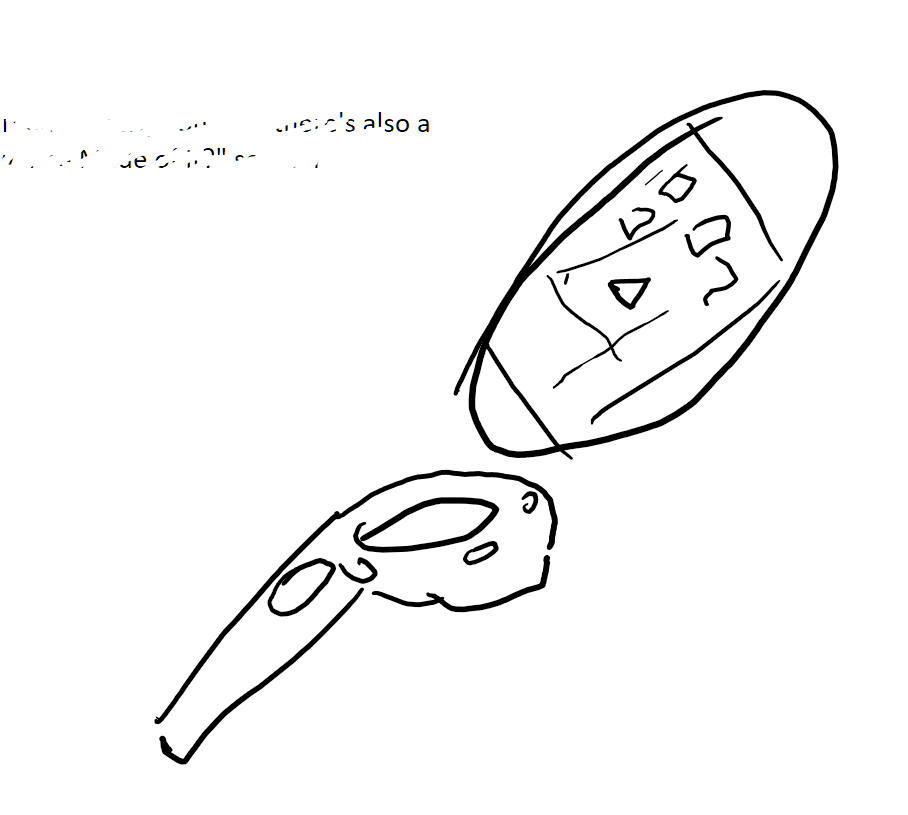
\includegraphics[width=0.7\linewidth]{figures/placeholders/minimap_controller}
	\caption{Controller with the minimap}
	\label{fig:minimap_controller}
\end{figure}


\paragraph{Gutwin vs our study}
% TODO: add a pic: Gutwin's (vertical) and our (horizontal) working (sound) plane
Since, this study extends upon \cite{gutwin_chalk_2011}, in this paragraph I provide a comparison of the two.
The main difference between - workspace is no longer a 2D plane, but an immersive 3D \gls{vr} environment. An important change here is the fact that participants are able to look around at the workspace, and notice some changes to the environment, even without the help of the minimap or auditory cues.
Second distinction is in the primary task of the participant and the simulated agent. In \cite{gutwin_chalk_2011} the participant performs the same task, as an agent: drawing with chalk. Additionally, the participant's actions emit the same sound (even though, at a lower volume) as the drawings of the agent. In this study, the primary task of the participant is - 3D drawing with voxels. This activity doesn't emit any sound. It is also different from the agent's task - translation of buildings in the urban district. Nevertheless, the tasks are still contextually related with regards to the architectural activity in urban environment.
\cite{gutwin_chalk_2011} do not specify the audio plane, in which the sound was simulated, in this experiment, the place was horizontal (TODO: ref figure). 

\begin{figure}[h]
	\centering
	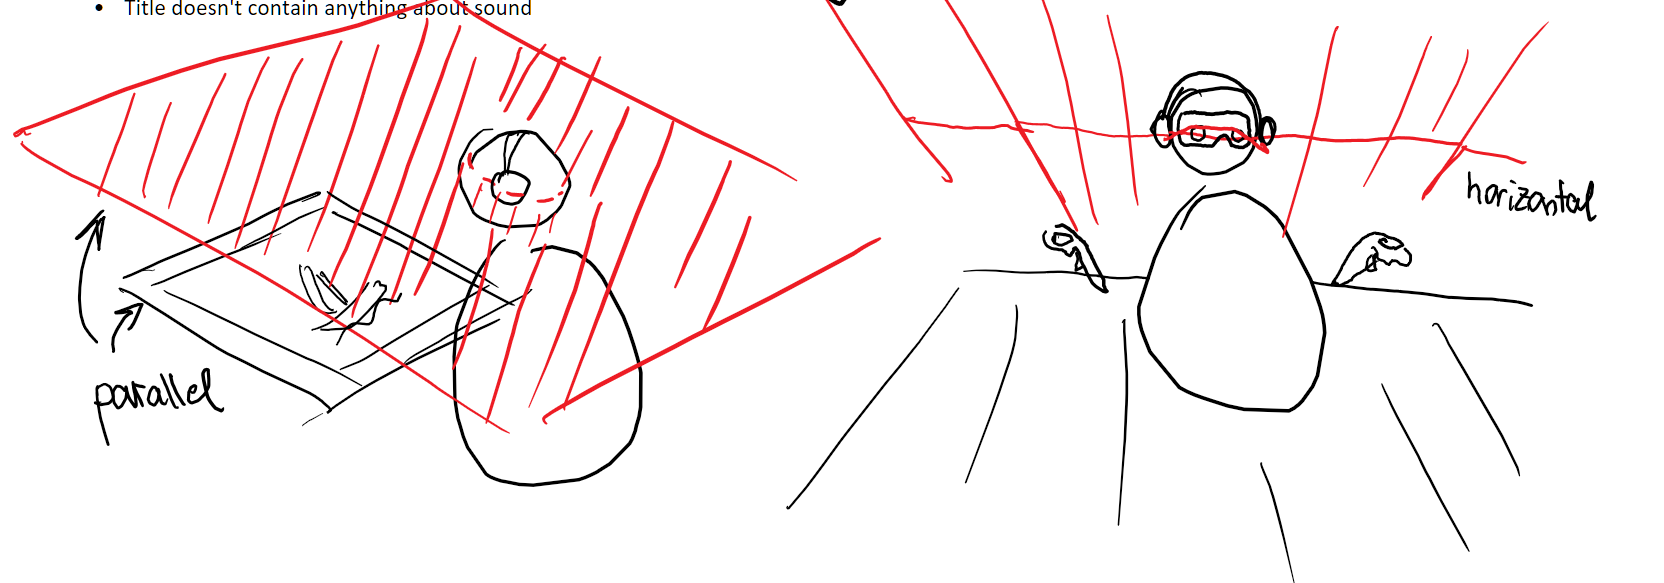
\includegraphics[width=0.7\linewidth]{figures/gutwin_vs_my_study_sound_plane}
	\caption{\cite{gutwin_chalk_2011} sound plane vs this study}
	\label{fig:gutwinvsmystudysoundplane}
\end{figure}


\begin{table}[]
  \caption{Study comparison: \cite{gutwin_chalk_2011} vs \gls{wa} in Immersive \gls{vr}}
  \label{table:study_comp}
  \begin{tabular}{|l|l|l|}
  \hline
                             & \cite{gutwin_chalk_2011}                & This study           \\ \hline
  Workspace dimensions				 & 2D									   & 3D \\ \hline
  Primary (distraction) task & The same as the primary for the simulated actor & Contextually related \\ \hline
  Working (sound) plane      & Variable             & Horizonatal          \\ \hline
  Sound type                 & Auditory icons        & Auditory icons       \\ \hline
  Object of analysis         & Workspace awareness   & Workspace Awareness  \\ \hline
  \end{tabular}
\end{table}

\paragraph{Results}

\paragraph{Study limitations}
% the fact that we only sample the level 1 SA/WA (we won't be going into sampling direction of translation guesses from the participants)
% could also try to describe it according to WA framework